\subsection{RAID}
Redundant array of independent disks (RAID) is originally designed as a visualization tool that establishes a whole storage space with multiple storage units. Different variation is developed to provide different level of data redundancy and I/O performance enhancement \cite{arpaci2012operating}. In a RAID system, a file is stripped and store in different physical disks depends on the actual variation. This characteristic makes RAID a natural strategy for distributed storage systems. These variations are \textit{levels}, known by 'RAID' followed by a level number. For example, the most common types of RAID are RAID 0, RAID 1 to RAID 6. Different levels of RAID are differ in their strategies in file striping, mirroring and parity computation. We focus on RAID 6 in this project.

By definition, RAID 6 refers to setup that is resilient to two arbitrarily disk failure. The resiliency here means it is capable of carry on read and write request to any logic disk in the RAID system. Figure \ref{fig:raid6} shows an example of a RAID 6 storage system with data blocks $A, B, C, D$ and $E$, each block is stripped into three parts (1-3) and two parities $p$ and $q$. In the example, parities are being stored in all available disks. An alternative scheme is to store $p$ segments and $q$ segments in two disks separated from the data parts. The parities are computed independently be performed by constructing and solving linear equations with one or two variables. 

\begin{figure}[t]
	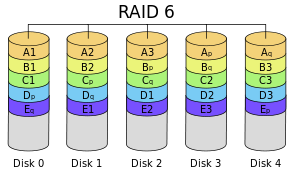
\includegraphics[width=9cm,height=5cm,angle=0]{RAID6.png}
	\caption{Diagram of a RAID 6 storage system with 3 block level data strippings and 2 parities \cite{wiki:raid} }
	\label{fig:raid6}
\end{figure}

\subsection{Galois field}
One of the parity is computed with a linear or $XOR$ 
Besides linearity, parity computations is preferred to be performed in a Galois field, or a finite field that the size of membership is limited to $p^k$, where $p$ is a prime number and $k$ is a positive integer. 

For example, the range of valid numbers in a Galois field $GF(2^8)$ is $0$ to $2^8-1=255$, and the 


\subsection{Reed-Solomen Coding}

In general, there are two main strategies to guarantee certain level of fault-tolerance. The first is full duplication, where all storage nodes have a independent mirror backup. In case of access failure, the backup copy can be used. The advantage of such design is, for a single fault, data recovery takes exactly the same read as the original request, incurring no additional read overhead. However, it is less cost-efficient, using only $1/2$ of the total hardware effectively in data storage. The second is using erasure coding